\documentclass[10pt]{beamer}
\usepackage{graphicx}
\usepackage{amsmath,amssymb,amstext,xargs,ifthen}
\usepackage{amsfonts}
\usepackage{bbm,tikz}
\usepackage{beamerthemesplit}
\usetikzlibrary{arrows}

\usepackage[utf8]{inputenc}
\usepackage[french]{babel}

\usetheme{Antibes}
\mode<presentation>
\useoutertheme{tree}
\usecolortheme{beaver}
\useinnertheme{rectangles}

\setbeamerfont{block title}{size={}}
%\usecolortheme[rgb={0.55,0.1,0.05}]{structure}
%\usecolortheme[rgb={0.75,0.1,0.05}]{structure}
\usepackage{color}
\def\rset{\mathbb{R}}

\def\1{\mathbbm{1}}
\def\mcb{\ensuremath{\mathcal{B}}}
\def\mcc{\ensuremath{\mathcal{C}}}
\def\mce{\ensuremath{\mathcal{E}}}
\def\mcf{\ensuremath{\mathcal{F}}}
\def\nset{\ensuremath{\mathbb{N}}}
\def\qset{\ensuremath{\mathbb{Q}}}
\def\rset{\ensuremath{\mathbb{R}}}
\def\zset{\ensuremath{\mathbb{Z}}}
\def\cset{\ensuremath{\mathbb{C}}}
\def\rsetc{\ensuremath{\overline{\rset}}}
\def\Xset{\ensuremath{\mathsf{X}}}
\def\Tset{\ensuremath{\mathsf{T}}}
\def\Yset{\ensuremath{\mathsf{Y}}}
\def\rmd{\mathrm{d}}
\def\Qint{\ensuremath{\mathrm{QInt}}}
\def\Int{\ensuremath{\mathrm{Int}}}
\def\eqdef{\ensuremath{\stackrel{\mathrm{def}}{=}}}
\def\eqsp{\;}
\def\lleb{\lambda^{\mathrm{Leb}}}
\newcommand{\rmi}{\mathrm{i}}
\newcommand{\rme}{\mathrm{e}}
\def\supp{\mathrm{supp}}
\newcommand{\Cov}[2]{\mathrm{Cov}(#1,#2)}


%notation fourier
\def\1{\mathbbm{1}}
\def\mcb{\ensuremath{\mathcal{B}}}
\def\mcc{\ensuremath{\mathcal{C}}}
\def\mce{\ensuremath{\mathcal{E}}}
\def\mcf{\ensuremath{\mathcal{F}}}
\def\nset{\ensuremath{\mathbb{N}}}
\def\qset{\ensuremath{\mathbb{Q}}}
\def\rset{\ensuremath{\mathbb{R}}}
\def\cset{\ensuremath{\mathbb{C}}}
\def\rsetc{\ensuremath{\overline{\rset}}}
\def\Xset{\ensuremath{\mathsf{X}}}
\def\Tset{\ensuremath{\mathsf{T}}}
\def\Yset{\ensuremath{\mathsf{Y}}}
\def\rmd{\mathrm{d}}
\def\Qint{\ensuremath{\mathrm{QInt}}}
\def\Int{\ensuremath{\mathrm{Int}}}
\def\eqdef{\ensuremath{\stackrel{\mathrm{def}}{=}}}
\def\eqsp{\;}
\def\lleb{\lambda^{\mathrm{Leb}}}
\newcommand{\coint}[1]{\left[#1\right[}
\newcommand{\ocint}[1]{\left]#1\right]}
\newcommand{\ooint}[1]{\left]#1\right[}
\newcommand{\ccint}[1]{\left[#1\right]}

\def\bu{\mathbf{u}}
\newcommand{\TF}{\mathcal{F}}
\newcommand{\TFC}{\overline{\mathcal{F}}}
\newcommand{\TFA}[1]{\mathcal{F}\left( #1 \right)}
\newcommand{\TFAC}[1]{\overline{\mathcal{F}}\left( #1 \right)}

\def\TFyield{\stackrel{\mathcal{F}}{\mapsto}}

\def\tore{\mathbb{T}}
\def\btore{\mathcal{B}(\tore)}
\def\espaceproba{(\Omega,\mathcal{A},\PP)}
\def\limn{\lim_{n \rightarrow \infty}}
\newcommand{\ps}{\ensuremath{\text{p.s.}}}
\newcommand{\pp}{\ensuremath{\text{p.p.}}}
\def\cA{\mathcal{A}}
\def\cC{\mathcal{C}}
\def\cL{\mathcal{L}}
\def\cM{\mathcal{M}}
\def\cN{\mathcal{N}}
\def\cO{\mathcal{O}}
\def\cP{\mathcal{P}}
\def\cS{\mathcal{S}}
\newcommand{\filtop}[1]{\operatorname{F}_{#1}}
\def\bfphi{{\boldsymbol{\phi}}}
\def\bfpsi{{\boldsymbol{\psi}}}
\def\bfgamma{{\boldsymbol{\gamma}}}
\def\bfpi{{\boldsymbol{\pi}}}
\def\bfsigma{{\boldsymbol{\sigma}}}
\def\bftheta{{\boldsymbol{\theta}}}
\def\bfhphi{{\hat{\boldsymbol{\phi}}}}
\def\bfhrho{{\hat{\boldsymbol{\rho}}}}
\def\bfhgamma{{\hat{\boldsymbol{\gamma}}}}

\def\ltwo{L_2}
\newcommand{\lone}{\ensuremath{L_1}}

\newcommand{\pltwo}{\ensuremath{\ell^2}(\zset)}
\newcommand{\plone}{\ensuremath{\ell^1}(\zset)}
\newcommand{\plinfty}{\ensuremath{\ell^\infty}(\zset)}
\newcommand{\plp}{\ensuremath{\ell^p}(\zset)}

\def\calG{\mathcal{G}}
\def\calM{\mathcal{M}}
\def\calI{\mathcal{I}}
\def\calH{\mathcal{H}}


\newcommand\BL[1]{\mathrm{BL}(#1)}%bande limit{\'e}e
%Espace de Schwarz
\def\mcs{\ensuremath{\mathcal{S}}}
%produit scalaire
\newcommand{\pscal}[2]{\left\langle #1, #2 \right\rangle}
\newcommand{\proj}[3][]{
\ifthenelse{\equal{#1}{}}{\ensuremath{\operatorname{proj}\left( \left. #2\right|#3\right)}}
{\ensuremath{\operatorname{proj}_{#1}\left( \left. #2 \right|#3\right)}}
}
%espaces engendr{\'e}s
\newcommand{\lspan}[1]{\mathrm{Vect}(#1)}
\newcommand{\cspan}[1]{\overline{\mathrm{Vect}(#1)}}
\def\oplusperp{\stackrel{\perp}{\oplus}}
\def\ominusperp{\ominus}%\def\ominusperp{\stackrel{\perp}{\ominus}}


%Operation sur les fonctions/distributions

\newcommand{\translation}{\mathcal{T}}
\newcommand{\multiplication}{\mathcal{M}}


%
\def\Rset{\mathbb{R}}
\def\Cset{\mathbb{C}}
\def\Zset{\mathbb{Z}}
\def\Nset{\mathbb{N}}
\def\Tset{\mathrm{T}}
% et d'autres
\newcommand{\vvec}[1]{\mathbf{#1}}
\newcommand{\signe}{\mathrm{sgn}}
\newcommand{\rect}{\mathrm{rect}}
\newcommand{\sinc}{\mathrm{sinc}}
\newcommand{\cov}{\mathrm{cov}}
\newcommand{\corr}{\mathrm{corr}}
\newcommand{\vp}{\mathrm{vp}}
\newcommand{\erf}{\mathrm{erf}}
\def\cF{\mathcal{F}}
\def\cE{\mathcal{E}}
\def\cB{\mathcal{B}}
\def\cH{\mathcal{H}}
\def\cG{\mathcal{G}}
\def\cI{\mathcal{I}}
\def\PP{\mathbb{P}}
\newcommand\PE[1]{{\mathbb E}\left[ #1 \right]}
\newcommand{\Var}[1]{\mathrm{Var}\left( #1 \right)}
\def\BB{\mathrm{B.B.}}
\def\BBF{\mathrm{B.B.F.}}
\newcommandx{\norm}[2][2=]{\left\Vert #1 \right\Vert_{#2}}
\newcommandx{\opernorm}[2][2=]{{\left\vert\kern-0.25ex\left\vert\kern-0.25ex\left\vert #1
    \right\vert\kern-0.25ex\right\vert\kern-0.25ex\right\vert}_{#2}}
\def\L1loc{L_{1,\mathrm{loc}}}
\def\Leb{\mathrm{Leb}}


\newcommandx\sequence[3][2=,3=]
{\ifthenelse{\equal{#3}{}}{\ensuremath{\{ #1_{#2}\}}}{\ensuremath{\{ #1_{#2}, \eqsp #2 \in #3 \}}}}
\newcommandx\sequencePar[3][2=,3=]
{\ifthenelse{\equal{#3}{}}{\ensuremath{\{ #1({#2})\}}}{\ensuremath{\{ #1({#2}), \eqsp #2 \in #3 \}}}}
\def\pp{\ensuremath{\mathrm{p.p.}}}
\def\ie{i.e.}

\newcommand{\ensemble}[2]{\left\{#1\,:\eqsp #2\right\}}
\newcommand{\set}[2]{\ensemble{#1}{#2}}
\def\retard{\operatorname{S}}
\def\foo{\rme^{-2 \rmi \pi \nu}}
\def\cfoo{\rme^{+2 \rmi \pi \nu}}
\def\toref{\coint{-1/2,1/2}} 
\title{MAP 555 : Discrete Fourier Transform...}
\begin{document}
\date{25 Septembre 2015}
\maketitle



\begin{frame}
\frametitle{Today}
\tableofcontents
\end{frame}

\section{Sampling}
\begin{frame}
\frametitle{Periodic sampling ?}
\begin{figure}
  \centering
  % Requires \usepackage{graphicx}
  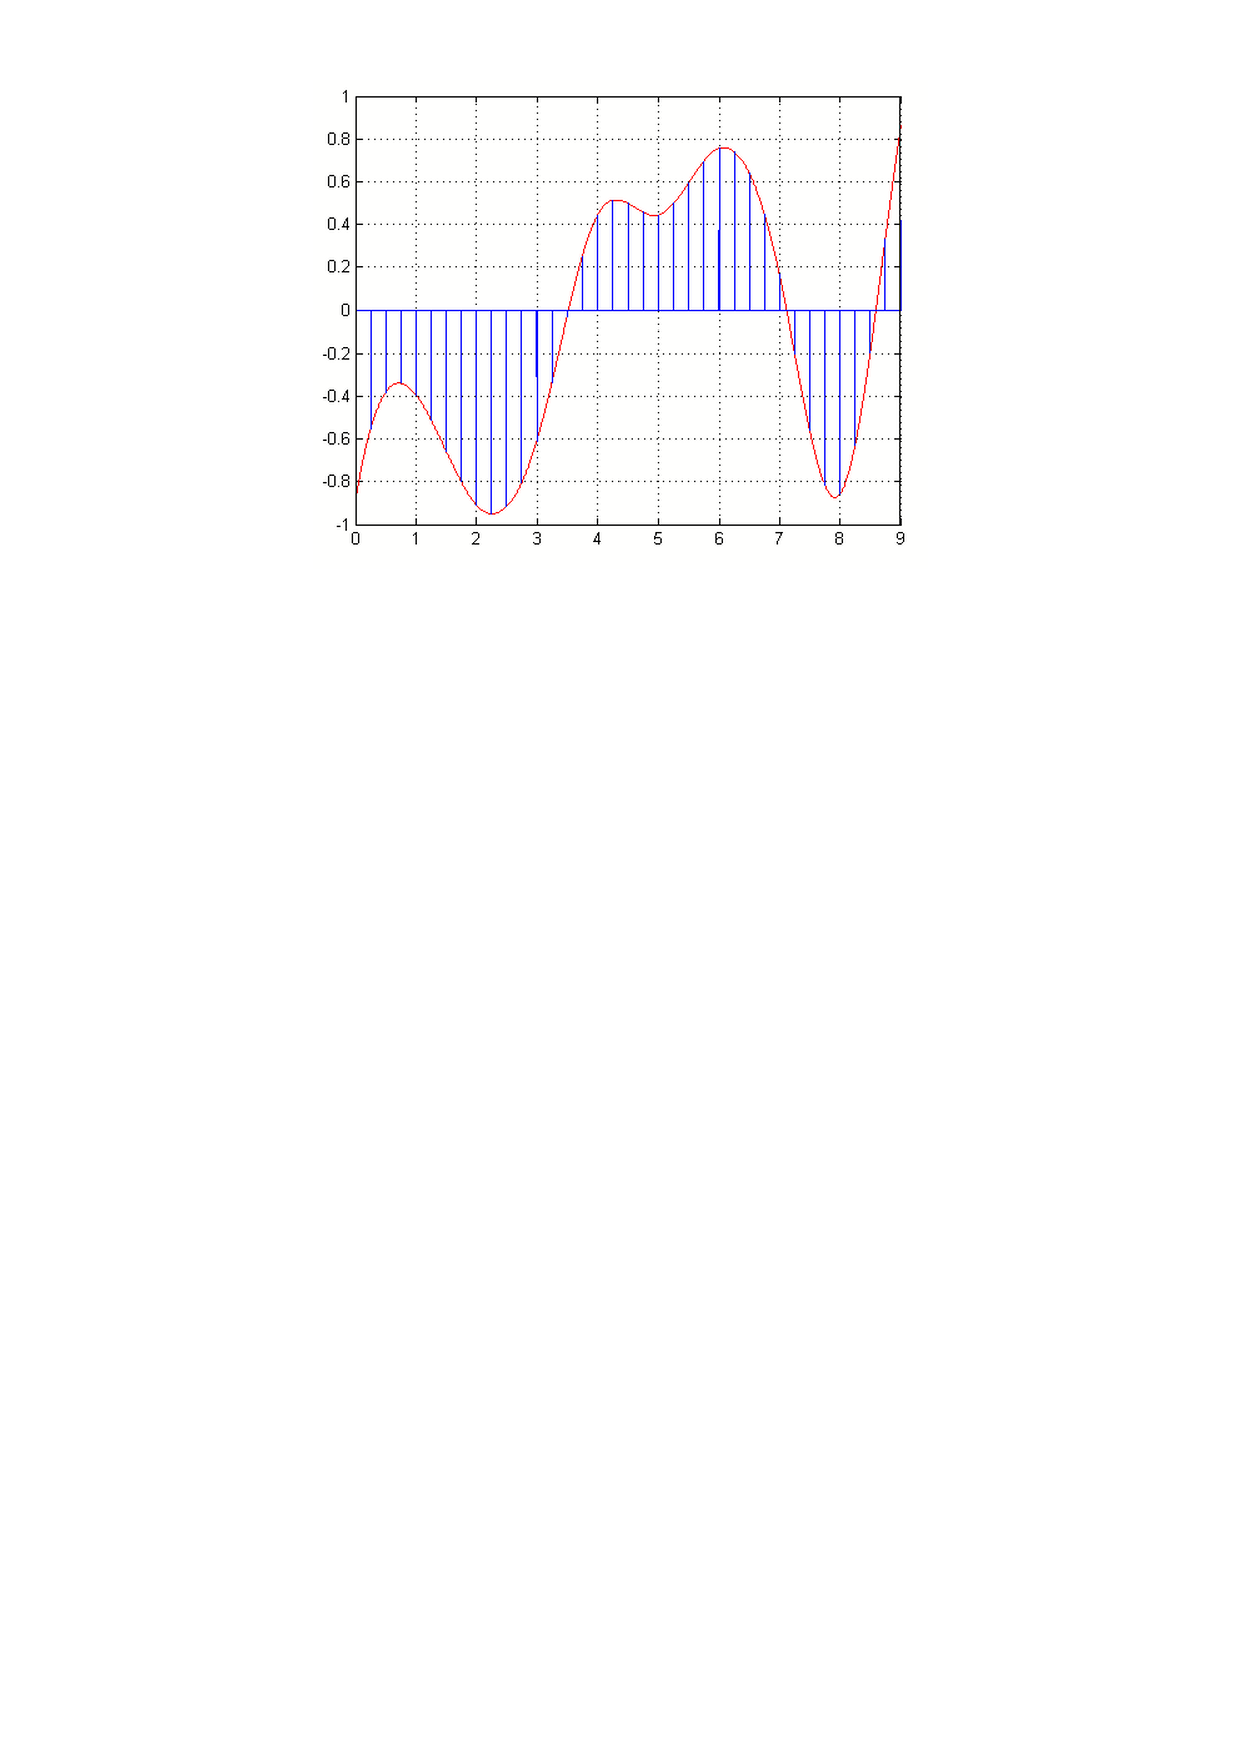
\includegraphics[width=0.6\textwidth]{sampling}\\
\end{figure}
\alert{$T$} the \alert{sampling period}. \alert{$f[n]= f(nT)$} are the samples of the signals.
The \alert{sampling frequency} \alert{$1/T$}.
\end{frame}


\begin{frame}
\frametitle{Band Limited functions}
\begin{definition}[Band Limited function]
A function $f \in L_2(\rset)$ is said to be  \alert{band limited} if there exists $B < \infty$ such that: $\TF f(\xi) = 0$ pour $\xi \not \in [-B,+B]$. We denote $\BL{B}$ the subspace of $f \in L_2(\rset)$ of functions satisfying $\TF f(\xi) = 0$ for (almost) all $\xi \not \in [-B,+B]$.
\end{definition}
\end{frame}

\begin{frame}
\frametitle{Band-Limited functions}
\begin{itemize}
\item The Fourier transform defines an isomporphism on $L_2(\rset)$. The inverse is $\TFC$.
\item Let  $f \in \BL{B}$. Since $\TF f$ is compactly supported and belongs $L_2(\rset)$, $\TF f  \in \lone(\rset)$.
\item Therefore $x \mapsto \TFC \circ \TF f(x)$ is continuous and since $\TFC \circ \TF f= f$ a.e., every function in $\BL{B}$ has a continuous version (and even a $C^\infty$ version).
\end{itemize}
\end{frame}

\begin{frame}
\frametitle{Periodizing the Fourier transform}
\only<1->{Let $T \leq 1/(2B)$ be the \alert{sampling period} and $1/T$ be the \alert{sampling frequency}.
Consider the periodic function $\xi \to \TF f(\xi)$ given by:
$$
F_T (\xi) = \sum_{n \in \zset} [\TF f] \left( \xi - \frac{n}{T} \right) \eqsp.
$$
}
\only<2>{$\xi \mapsto F_T(\xi)$ is periodic with period $1/T$}
\only<3>{The function  $F_T \in L_2{[-1/2T,1/2T]}$ can be expanded as a series function
\begin{equation*}
F_T (\xi) = \sum_{n \in \zset} c_n(F_T) \rme^{- \rmi 2 \pi \xi n T},
\end{equation*}
where $\{c_k(F_T)\}$, the Fourier coefficients are given by
\begin{equation*}
c_k(F_T) = T \int_{-1/(2T)}^{1/(2T)} F_T(\xi) \rme^{+ \rmi 2 \pi \xi k T} \rmd \xi\eqsp.
\end{equation*}
}
\end{frame}

\begin{frame}
\frametitle{Periodizing the Fourier transform}
The identity
\begin{equation*}
F_T (\xi) = \sum_{n \in \zset} c_n(F_T) \rme^{- \rmi 2 \pi \xi n T},
\end{equation*}
should be understood as a convergence of the partial sums
\begin{equation*}
F_{N,T}(\xi)= \sum_{k=-N}^N c_N(F_T) \rme^{- \rmi 2 \pi \xi n T} \eqsp,
\end{equation*}
toward $F_T$ in the topology induced by the norm $\|\cdot\|_2$  in $L_2([-1/(2T),1/(2T)])$:
$$
\lim_{N \to \infty} \int_{-1/(2T)}^{1/(2T)} |F_T(\xi) - F_{N,T}(\xi)|^2 \rmd \xi =0 \eqsp.
$$
\only<2>{The Parseval identity implies that $\sum_{n \in \zset} |c_n(F_T)|^2 < \infty$}.
\end{frame}

\begin{frame}
\frametitle{A key result}
\begin{itemize}
\item Since for all $T \leq 1/(2B)$, $[-B,+B] \subset [-1/(2T), 1/(2T)]$, then for all $\xi \in [-1/(2T),1/(2T)]$,
\alert{
$$F_T(\xi) = \TF f(\xi) $$
}
\item Therefore, the  Fourier coefficients $c_k(F_T)$ are given by:
\alert{
\begin{equation*}
c_k(F_T) = T \int_{-B}^{B} \TF f(\xi) \rme^{+ \rmi 2 \pi \xi k T} \rmd \xi= T f(kT)\eqsp.
\end{equation*}
}
\end{itemize}
\end{frame}



\begin{frame}
\frametitle{The Poisson Formula: Key result}
If $f \in \BL{B}$ then the \alert{discrete-time Fourier transform} (DTFT) of the sequence of samples $\{ f(nT), n \in \zset \}$
\[
T \sum_{n \in \zset} f(nT) \rme^{- \rmi 2 \pi \xi n T}
\]
is equal to the Fourier transform of the function $f$ periodized with a period $1/T$, a relation called the \alert{Poisson formula}
\begin{equation*}
\label{eq:FormuleSommatoirePoisson}
\sum_{n \in \zset} \TF f \left( \xi - \frac{n}{T} \right)  = T \sum_{n \in \zset} f(nT) \rme^{- \rmi 2 \pi \xi n T}\eqsp,
\end{equation*}
\only<2>{An amazing result: the DTFT is computable only from the knowledge of the samples $\{x(nT), n \in \zset\}$, whereas
the knowledge of $\TF f$ requires to evaluate the function at all time points
}
\only<3>{the DTFT is periodic with period $1/T$, which is the sampling frequency. Because of this periodicity, one may restrict the frequency
interval to just one-period, $[-1/2T,1/2T]$}
\end{frame}

\begin{frame}
\frametitle{Interpolation formula}
\begin{itemize}
\item \alert<1>{Multiply the Poisson formula
\begin{equation*}
\sum_{n \in \zset} \TF f \left( \xi - \frac{n}{T} \right)  = T \sum_{n \in \zset} f(nT) \rme^{- \rmi 2 \pi \xi n T}\eqsp,
\end{equation*}
by the indicator function $\1_{[-1/(2T),1/(2T)]}(\xi)$}
\item \alert<2>{Use the identity $$\1_{[-1/(2T),1/(2T)]}(\xi) \TF f (\xi)= \1_{[-1/(2T),1/(2T)]}(\xi) F_T(\xi)$$}
\end{itemize}

\end{frame}

\begin{frame}
\frametitle{Interpolation formula}
For all $\xi \in [-1/2T,+1/2T]$,
$$
\TF f (\xi) = T \sum_{n \in \zset} f(nT) \1_{[-1/(2T),1/(2T)]}(\xi) \rme^{- \rmi 2 \pi \xi n T} \eqsp.
$$
which should be understood as
$$
\lim_{N \to \infty} \int \left| \TF f(\xi)  - T \sum_{n =-N}^N f(nT) \1_{\left[-\frac{1}{2T},\frac{1}{2T}\right]}(\xi) \rme^{- \rmi 2 \pi
    \xi n T}  \right|^2 \rmd \xi = 0 \eqsp.
$$
Since $\TFC$ is an isometry and $\TFC \TF f = f$ a.e.
$$
\lim_{N \to \infty} \int \left| f(t)  - T \sum_{n =-N}^N f(nT) \TFAC{\1_{\left[-\frac{1}{2T},\frac{1}{2T}\right]}(\xi) \rme^{+ \rmi 2 \pi
    \xi n T}}(t) \right|^2 \rmd t = 0 \eqsp.
$$
\end{frame}

\begin{frame}
\frametitle{Interpolation formula}
\begin{lemma}
$$
\TFAC{\xi \to \1_{[-1/(2T),1/(2T)]}(\xi) \rme^{+ \rmi 2 \pi \xi n T}}(x)= \frac{\sin\left( \frac{\pi}{T}(x - nT)\right)}{\pi(x-nT)}
$$
\end{lemma}


\end{frame}

\begin{frame}
\frametitle{Interpolation formula}
\begin{theorem}[Nyquist theorem]
If $f \in \BL{B}$ and $T \leq 1/2B$ then
\alert{
\begin{equation*}
f(x) =_{\ltwo(\rset)} \sum_{n \in \zset} f(nT) s_T(x-nT)  \eqsp,
\end{equation*}
}
where $s_T$, is the cardinal-sine function
\alert{
$$
s_T(x) = \frac{\sin \left( \pi x/T\right) }{ \pi x/T}\eqsp.
$$
}
If in addition,
$$
\sum_{k \in \zset} |f(kT)| < \infty,
$$
the series converges uniformly to $f$.
\end{theorem}
The condition  \alert{$T \leq 1/2B$} is the \alert{Nyquist condition}.
\end{frame}

\section{Frequency resolution and windowing}

\begin{frame}
\frametitle{From theory to practice}
\begin{itemize}
\item Even though $T\sum_{k=-\infty}^{\infty} f(kT) \rme^{-\rmi 2 \pi \xi kT}$ is the closest approximation  of $\TF f$ that we can achieve digitally, it is still not computable because generally it requires an \alert{infinite number of samples}.
\item To make it computable, we must make a \alert{second approximation}, keeping only a \alert{finite number} of samples $\{ f(kT), 0\leq k \leq L-1\}$ (assuming a \alert{causal} signal).
\item In terms of the times samples, the \alert{time windowed version} is given by
\[
T \sum_{k=0}^{L-1} f(kT) \rme^{- \rmi 2 \pi \xi kT}  
\]
\end{itemize}
\end{frame}

\begin{frame}
\frametitle{Normalized frequency}
\begin{itemize}
\item It is customary to define the \alert{normalized} frequency as \alert{$ \lambda = \xi/ \xi_s$}, where \alert{$\xi_s= 1/T$} is the sampling frequency. 
\item Expressed in terms of the normalized frequency $\lambda$, the discrete time Fourier transform is given by
\[
\lambda \mapsto \sum_{k=-\infty}^{\infty} f(kT) \rme^{- \rmi 2 \pi k \lambda}
\]
which is periodic with period $1$. It is customary to represent this function on the interval $\ccint{-1/2,1/2}$.
\item It is sometimes more appropriate to work with the \alert{normalized pulsation} \alert{$\omega= 2 \pi \lambda$}.
\item In the sequel we set conventionally $T=1$   
\end{itemize}
\end{frame}

\begin{frame}
\frametitle{From theory to practice}
\begin{itemize}
\item The windowed signal may be thought of as an \alert{infinite sequence} which is zero outside the range of the window and agrees with the original one within the window. 
\item To express this mathematically, we define the \alert{rectangular} window of length $L$:
\[
w(n) = 
\begin{cases}
1 \eqsp & n \in \{0,\dots,L-1\} \\
0 &  \text{otherwise}
\end{cases}
\]
\item The Discrete time Fourier transform of the windowed signal $\{ w(n) f(n), n=0,\dots,L-1\}$ is given by
\[
F_L(\omega)= \sum_{k=0}^{L-1} w(k) f(k) \rme^{-\rmi \omega k} \eqsp.
\]
\item As the window length $L$ increases, the windowed DTFT becomes a better approximation of the DTFT
\[
F(\omega) = \sum_{k=-\infty}^{\infty} f(k) \rme^{-\rmi \omega k} \eqsp,
\]
and is computable for any value of the pulsation $\omega$.
\end{itemize}
\end{frame}

\begin{frame}
\frametitle{Windowing effect}
\begin{itemize}
\item In general, the windowing process has two major effects: 
\begin{enumerate}
\item First, it reduces the \alert{frequency resolution} of the computed spectrum, in the sense that the \alert{smallest resolvable frequency difference is limited by the length of the data record, that is, $\Delta f =1/(2 L+1)$. This is linked with the \alert{uncertainty principle.}
 \item Second, it introduces \alert{spurious} high-frequency} components into the spectrum, which are caused by the sharp clipping of the signal at the left and right ends of the rectangular window. This effect is referred to as \alert{frequency leakage.}
\end{enumerate}
\item Both effects can be understood by deriving the precise connection of the windowed DTFT  to the unwindowed DTFT.
\end{itemize}
\end{frame}

\begin{frame}
\frametitle{Convolution}
\begin{itemize}
\item Recall that $f(n)$ is the $n$-th Fourier coefficient of the $\pi$-periodic function $F(\omega)$
\[
f(n) = \frac{1}{2 \pi} \int_{-\pi}^{\pi} F(\omega') \rme^{+ \rmi \omega' n} 
\]
\item Hence, we get 
\begin{align*}
\sum_{n=-\infty}^{\infty} x(n) w(n) \rme^{-\rmi \omega n} &= (2 \pi)^{-1} \sum_{n=-\infty}^{\infty} w(n) \int_{-\pi}^{\pi} X(\omega') \rme^{-\rmi (\omega-\omega') n} \rmd \omega' \\
&= (2\pi)^{-1} \int_{-\pi}^\pi X(\omega') W(\omega - \omega') \rmd \omega'
\end{align*}
where $W(\omega)$ is the DTFT of the window
\[
W(\omega)= \sum_{k=0}^{L-1} w(n) \rme^{-\rmi \omega n} \eqsp.
\]
\end{itemize}
\end{frame}

\begin{frame}
\frametitle{Fourier transform of a rectangular window}
\begin{itemize}
\item The DTFT of the recatngular window is given by 
\[
\sum_{k=0}^{L-1} \rme^{-\rmi \omega k}= \frac{\sin(\omega L/2)}{\sin(\omega/2)} \rme^{- \rmi \omega (L-1)/2}
\]
\item The function has a maximum at $0$ which is equal to $L$ and is $\pi$ periodic.
\end{itemize}
\end{frame}

\begin{frame}
\begin{figure}
  \centering
  % Requires \usepackage{graphicx}
  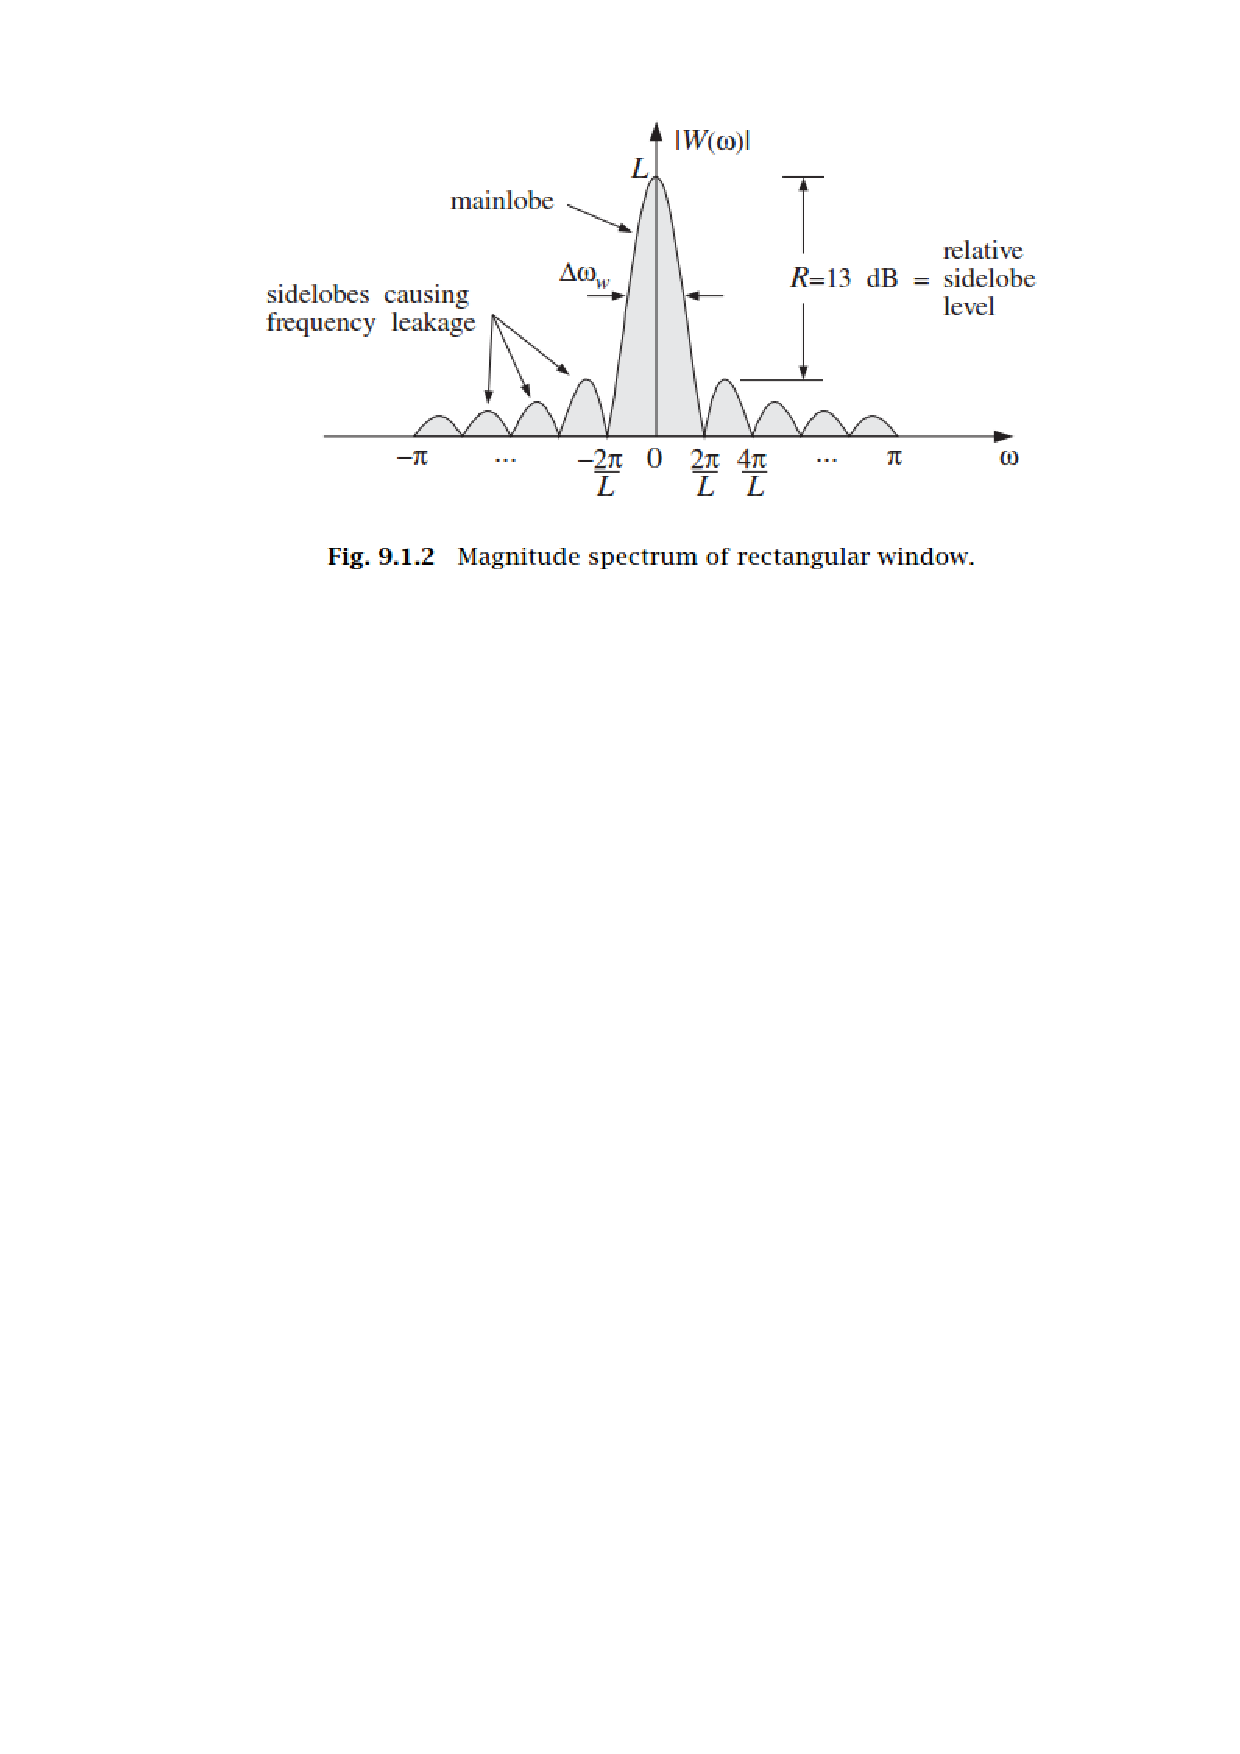
\includegraphics[width=0.7\textwidth]{rectangularw}\\
\end{figure}
\end{frame}

\begin{frame}
\frametitle{Mainlobes and sidelobes}
\begin{itemize}
\item It consists of a \alert{main lobe} of height $L$ and base width $4\pi/L$ centered at $\omega=0$, and several smaller \alert{sidelobes}.
\item The sidelobes are between the zeros of $W(\omega)$ , which are the zeros of the numerator $\sin(\omega L/2)=0$, that is, $\omega=2\pi k/L$, for $k=\pm 1, \pm 2,\ \ldots$ (with $k=0$ excluded).
\item The mainlobe peak at $0$ dominates the spectrum, because $w(n)$ is essentially a low-pass  signal, except when it cuts off at its endpoints.
\item The higher frequency components that have `leaked'' away from $0$ and lie under the sidelobes represent the sharp transitions of $w(n)$ at the endpoints.
\item The \alert{width} of the mainlobe can be defined in different ways. For example, we may take it to be the width of the base, $4\pi/L$, or, take it to be the 3-dB width, that is, where $|W(\omega)|^{2}$ drops by 1/2.
\end{itemize}
\end{frame}

\begin{frame}
\frametitle{Mainlobes and sidelobes}
\begin{itemize}
\item  For simplicity, we  define the width of the mainlobe  to be half the base width, that is, in units of radians per sample:
$$
\Delta\omega_{w}=\frac{2\pi}{L} \quad \text{(rectangular window width)}
$$
\item In units of Hz, it is defined through $\Delta\omega_{w}=2\pi\Delta \xi_{w}/\xi_{s}$:
$$
\Delta \xi_{w}=\frac{\xi_{s}}{L}=\frac{1}{LT}=\frac{1}{T_{L}}\
$$
\item We will see shortly that the mainlobe width $\Delta \xi_{w}$ determines the {\it frequency resolution limits} of the windowed spectrum. As $L$ increases, the height of the mainlobe increases and its width becomes narrower, getting more concentrated around 0. 
\item However, the height of the sidelobes also increases, but \alert{relative} to the mainlobe height, it remains approximately the same and about 13 dB down.
\end{itemize}
\end{frame}

\section{The Discrete Fourier Transform}

\end{document} 